\RequirePackage{ifpdf}
\documentclass[a4paper,11pt,openany]{kth-mag}
%\let\ifpdf\relax
\usepackage[T1]{fontenc}
\usepackage{textcomp}
\usepackage{lmodern}
\usepackage[latin1]{inputenc}
\usepackage[swedish,english]{babel}
\usepackage{modifications}
\usepackage{graphicx}
\usepackage{amsmath}
\usepackage{times}
\usepackage{subfigure}
\usepackage{multirow}
\usepackage{colortbl,booktabs}
\usepackage{todonotes}
\usepackage{color}

\title{Prediction of peptide retention time based on Gaussian Processes}


\foreigntitle{}
\author{XuanBin Qiu}
\date{March 2015}
\blurb{Master's Thesis at NADA\\
External Supervisor: Lukas K\"{a}ll\\
Internal Supervisor: Patric Jensfelt\\
Examiner: Stefan Carlsson}
\trita{TRITA 2015-3-19}

\begin{document}
\frontmatter
\pagestyle{headings}
\removepagenumbers
\maketitle
\selectlanguage{english}
\begin{abstract}
 \todo[inline]{Re-write the abstract with respect to things we have corrected in the thesis.}
  Retention time (RT) as an important evidence can be used to analysis the peptide's properties. Because of the interactions among peptides, the retention time prediction of peptide has low accuracy,
  and thus is less effective in the validation of peptide identifications. Besides, the large amount of time on generating features also need to be reduced. This thesis presents a alternative machine learning methods to predict the retention time of a set of peptide in hand. In order to address the precision and computational cost problem, we introduce Gaussian Processes as the trained model and use a new feature extraction method called BOW to generate the features for training the model. We also investigate the effect of different types of kernel function and their parameters. The results show high precision of the prediction and relatively low time cost.
\end{abstract}

\clearpage
\tableofcontents*

\mainmatter
\pagestyle{newchap}
\chapter{Introduction}
\fontsize{12pt}{16pt}\selectfont

\section{Introduction}

Protein, the most essential component of all the cells and organisms, plays an irreplaceable role in people's daily lives including providing energy, strengthening the immune system and catalyzing metabolic reactions within the body. Functions of different biological organisms are determined by the proteins that are presented in them. For this reason, it is important and necessary for us to know what proteins are in different organisms. As a result, this leads us to the problem of large-scale identification of proteins in complex mixtures.

\begin{figure}[h!]
  \centering
  % Requires \usepackage{graphicx}
  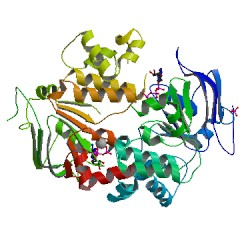
\includegraphics[width=0.3\textwidth]{./figures/protein.jpg}\\
  \caption{protein chain}\label{fig:protein}
\end{figure}

\begin{figure}[h!]
  \centering
  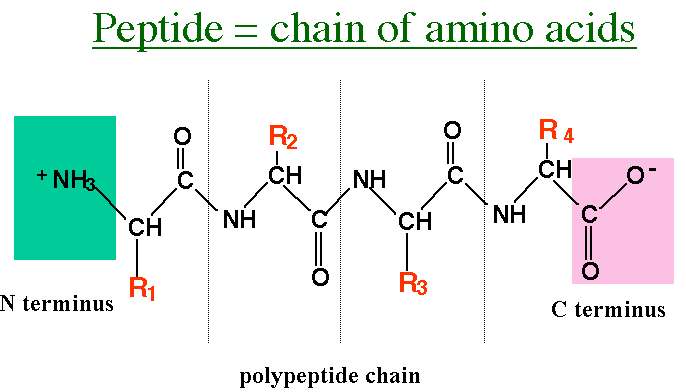
\includegraphics[width=0.4\textwidth]{./figures/peptide.png}\\
  \caption{Peptide model}\label{fig:Fig3}
\end{figure}
\noindent
Shotgun proteomics \cite{fooa}\cite{foob} is the most popular technique for identifying proteins in complex mixtures. The main part of this technique is high performance liquid chromatography (HPLC). HPLC has three main steps, firstly, the protein in the mixture of interest will be broken into peptides. A peptide is a short sequence (chain) of amino acid as in Fig.\ref{fig:Fig3}. Then the resulting peptides are separated according to their hydrophobicity on a thin tube called liquid chromatography (LC) column. The hydrophobicity is the physical property of a molecule that is seemingly repelled from a mass of water. To be more specific, a specific solvent will be pumped through the column with increasing concentration. Peptide with different hydrophobicity will gradually digest in the solvent due to their hydrophobicity and then wash out from the column.\\

\noindent
In the end, those peptides will separated from the column and ionized by electrospray ionization and then tossed into mass spectrometer. The result is a set of spectra. Each spectra corresponds to only one or at most a few specific peptides. The fig.\ref{fig:HPLC} shows the general process of HPLC method.\\

\begin{figure}[h!]
  \centering
  % Requires \usepackage{graphicx}
  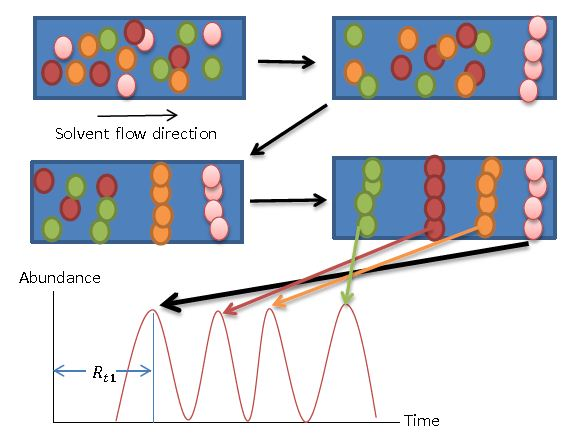
\includegraphics[width=0.5\textwidth]{./figures/RPLC_flow.jpg}\\
  \caption{Demonstration of HPLC method. (circles with different colour represents different peptides and the blue column represents the liquid chromatography column, The $R_{t1}$ is the retention time of $peptide Pink$)}\label{fig:HPLC}
\end{figure}

\noindent
Since we want to know which peptides were in the sample, we will compare them with a list of theoretical peptides from the database that we know should be in the sample. Currently, we have to compare every peptide with every spectrum to see if the peptide exists in the sample or not. However, when the number of peptides becomes increasingly large, the complexity of this method becomes extremely high which will result in a poor computational efficiency.\\

\noindent
An alternative way to solve this problem is to utilize its retention time. We could reduce the number of peptides compared to a spectrum if we know which peptides are more likely to separated from the column at the time the spectrum is produced. This time is defined as the retention time of a peptide. So the more precise the predicted retention time we could get, the less peptides we need to match and the higher efficiency we could have to identify the peptide.\\


\section{Problem Statement}

\noindent
Different models have been applied to the task of predicting the retention time of the peptides. For example, the Sequence Specific Retention Calculator (SSRC) which predicts retention times based on amino acid sequences is available on-line \cite{foo15}.\\

\noindent
To train a regression model, we first need some proper features which can represent the peptide in a vector space. Since most of most of the available features are biochemical features, we are interested in BOW features that have shown to be successful for sequence analysis. Therefore, in this thesis will utilize these features for training model and compare their performance to the traditional biochemical features.\\

\noindent
The main algorithm behind current RT prediction methods is mostly based on either Support Vector Regression (SVR) or Artificial Neural Network (ANN) and all of these methods have their own drawbacks that need to be improved.\\

\noindent
In this thesis, we would like to apply the Gaussian Processes (GP) model to predict the retention time and investigate its performance by comparing it with the other existing methods.\\

\noindent
GP provides a flexible framework for probabilistic regression and is widely used to solve high-dimensional, small-sample or nonlinear problems. Yet none of the existing publications has used this model for predicting retention times.\\

\noindent
In addition, since GP model has some parameters need to be optimized which have a significant impact on the prediction accuracy, in this thesis, we will investigate different optimization methods towards these parameters and analyze their properties. \\


\section{Outline}


The structure of the thesis is as following: Chapter 2, introduces the related works. Chapter 3, provides the whole methodologies and is divided into 3 sections, section 1 provides the detailed description of Gaussian Processes and a detailed mathematics derivation and section 2 gives the idea of Bag of word method for features selection and section 3 will cover the two optimization methods that are used to optimize the parameters of our model. Chapter 4, the experimental results and evaluation will be analyzed and our model will be compared with some other popular predictors. Chapter 5, a discussion of the limitation of our model will be given. Chapter 6, discusses the future work and gives some perspectives for it.



\chapter{Related Work}
\fontsize{12pt}{16pt}\selectfont
\noindent
Prediction of the retention time for a given peptide could help to improve the confidence of peptide identification. \textcolor{red}{Therefore, developing efficient algorithms and establishing proper models to generate the prediction of peptide has become more important and necessary.}\\
\todo[inline]{Therefore, it is import and necessary to develop .... to ...}


\todo[inline]{To design a successful predictor for our task, one would has the following questions. (not two problems) - Rewrite this paragraph}
\noindent
\textcolor{red}{However,}\todo{remove} to make the prediction successfully, there are two problems needed to be considered. Firstly, what kind of model will have better performance of the prediction\todo{this is a question so end it with ?}. Secondly, what factors will have a great impact on the retention time\todo{same here end with ?}. \textcolor{red}{Unfortunately, both of these two questions remain open so far. Therefore,}\todo{Remove} in order to answer the questions, a number of models based on different features have been proposed to characterize \textcolor{red}{quantitatively the peptide}\todo{This is strange find a better wording.} and to predict its retention time.\\

\section{Models / Methods}
\noindent
\todo[inline]{Maybe : Different machine learning models have been applied to the task of predicting peptide retention time. In \cite{?},  Baczek T \textit{et al.} have implemented }

\todo[inline]{Re-write this section with this format : In [paper citation], First author \textit{et al.} have implemented [ this model ]. Then describe the properties of what they have done. }


\textcolor{red}{There are}\todo{remove} different kinds of \textcolor{red}{machine-learned models}\todo{machine learning models} \textcolor{red}{that}\todo{remove} have been implemented. One of the model is the multiple linear regression (MLR) model. This model was implemented by Baczek T, Wiczling P, Marszall M, et al in \cite{foo1} to predict the peptide retention time at different HPLC conditions and shows high precision. However, the linear regression model mainly depends on the chromatographic condition and thus prediction bias could be a serious problem when the model is used under different circumstances. \\

\noindent
Another model is the artificial neural network(ANN) proposed by Petritis K et al. in \cite{foo2}. The ANN model was based on the contributions of individual amino acids taken the neighborhood effect into account and a data set of 7000 was used for the training. The large amount of experimental data provided by this approach produced high accuracy of the retention time prediction and enhance the confidence of the peptide identification. In \cite{foo3}, Petritis K, Kangas LJ, Yan B, et al have improved the ANN model by adding more descriptors, such as peptide length, sequence, hydrophobicity as well as nearest-neighbor amino acid. Each of the peptide is characterized by 1052 features instead of 20. The new model was trained by 345,000 peptide and tested using another 1303 confidently identified peptide which reported excellent performance.\\


\todo[inline]{It is not clear at all what model you are talking about in the next paragraph!}
\noindent
Although a great deal of effort has been made \textcolor{red}{to improve the model}\todo{into improving the models}, there are still some remaining issues. One of the main weaknesses of this model is its time consumption. In order to train this model, a large amount of training data is required which will result in a high cost in terms of both time and resources. What's worse, its high computational cost also implies its weakness in terms of repeatability and comparability which are essential to laboratory research. It also limits its development for commercial purpose.\\

\noindent
In order to solve this problem, another alternative machine-learning method, support vector machine(SVMs) has been implemented. Klammer et al. in \cite{foo4} proposed a predictor based on this method. \textcolor{red}{SVMs requires fewer data to train the model than ANNs}\todo{Compared to ANNs, SVMs require a smaller training set which can reduce the ...} and reduce the computational cost dramatically. Besides, dynamic SVR (support vector machine for regression problem) model avoids the RT variation between different chromatographic conditions which could have better performance than the linear regression model in terms of adaptability. However, using small dataset with low complexity to train the model also leads to the poor performance in terms of accurate regression and gives lower quality prediction compared to the ANNs. \textcolor{red}{If we simply use the same amount of the training data as in ANNs, the SVR model could have better performance but with extremely high computational cost which might even worse than ANNs.}\todo{Re-write this sentence.}\\


\noindent
To enhance the capacity of the predictor and raise the predicted accuracy, Luminita Moruz\todo{ \textit{et al.} } in \cite{foo5} has developed a new predictor, ELUDE, \todo{which is based}  based on support vector regression (SVR). The predictor firstly derives a retention time index for the condition at hand. Then by using those indices, the predictor creates 60 peptide features which are optimally combined during a second training procedure. After that, $\epsilon-SVR$, \textcolor{red}{a popular kind of SVR model}\todo{remove}, is used to train the model based on the features. The resulting retention model can be subsequently used to predict the retention time of other peptides of interest. \\

\noindent
The performance of Elude is excellent and considered as one of the state-of-the-art retention time predictors. However, one of the shortcomings of the Elude algorithm is the rather limited use of positional information. The positional information here is mainly about the relative position of different amino acids in the peptide. \textcolor{red}{The retention index trained in-house on which many of the other features are based is calculated using only the amino acid composition.}\todo{Re-write} Adding positional data is likely to capture more information, and thus lead to higher prediction accuracies\todo{accuracy} \cite{foo6}.\\


\todo[inline]{Re-write the following paragraph. If this happens then the results will be bad.}
\noindent
However, even with the proper models, the prediction could fail or the precision could be extremely low if the selected features are improper or unrepresentative. So the features selection is also a essential part of an successful prediction.\\

\section{Features}
\noindent
The effect of an individual amino acid was firstly taken into account when building the model because \textcolor{red}{evidences implied}\todo{evidence has implied} that the inclusion of this type of additional information could increase the confidence of \textcolor{red}{protein identification of the peptide}\todo{peptide indetification} \cite{foo1} and the chromatographic behavior of a peptide is mainly dependent on its amino acid composition \cite{foo7}\todo{reverse these, peptides are composed of amino acids and it can increase the performance}. A set of retention time coefficients were generated from only different amino-acid composition by using iterative regression methods \cite{foo8} \cite{foo9} \cite{foo10} \todo{explain the last sentence more.}.\\

\todo[inline]{In \cite{foo9}, it is pointed out that ... }
\todo[inline]{change every thing below that you have, the author of ..., write them like Author \textit{et al.} in \cite{?} have also emphasized .. }
\noindent
However, the author of \cite{foo9} pointed out that the relative location of different amino acid\todo{amino acids} in a peptide could affect the behavior of the peptide too. The author of \cite{foo11} has also emphasized the relation between the chromatographic behavior of peptides and their amino acid composition. \textcolor{red}{It is for sure that different values of retention coefficients of the same amino acid need to be assigned according to different peptides and different neighborhoods.}\todo{Re-write} Besides, \textcolor{red}{the}\todo{remove} other biological characters, such as hydrophobicity \cite{foo12}, ion-pairing reagents \cite{foo13}, stationary phase \cite{foo14} and even the length of the peptide could influence the peptide retention \textcolor{red}{behavior}\todo{time}. \\

\noindent
\textcolor{red}{Thus,}\todo{remove} in \cite{foo15}, O.V. Krokhin and R. Craig have developed an improved model, Sequence-Specific Retention Calculator(SSRC), for prediction of retention times in ion pair reversed-phase based on a database of 346 peptides. The ability of this model for prediction can assist detailed peptide mapping significantly, thus increase confidence in peptide identification and the protein characterization. However, the model is not completed and has not included amino acid modification that may occur during the sample preparation. In addition, the prediction capacity becomes worse for \todo{an experimental condition} experimental condition which \textcolor{red}{is diverging}\todo{diverges} from the setup.\\

\todo[inline]{Again write, In \cite{?}, the authors have ... }

\noindent
After SSRC, several different kinds of factors have been used. One of them is the structural descriptors. The author \todo{who is the autho?} has employed the Quantitative structure-retention relationships with the information of the peptide's chemical characters and its structure in article \cite{foo16}. The predictor implemented in \textcolor{red}{article}\todo{Remove} \cite{foo1} is also based on three types of chemical structural descriptors and both of them showed good results with the experimental data.\\

\noindent
In general, most of the features that are widely used \textcolor{red}{now}\todo{remove} have strong biological meaning, such as amino acid composition, hydrophobicity of the peptide and some other chemical structural descriptors and the performances of these features could fulfill the requirement. However, few of the less-biological meaning features have been tried so far. \\

\noindent
From the perspective of computer science, anything that can represent an object could be considered as a feature of this object. Therefore, it is worth to believe that some less-biological meaning features could give the same performance in this case. It might be a breakthrough to introduce some new features instead of just using the biochemical features. In this thesis,  some features with less biological meaning will be utilized and compared to the traditional biochemical features.


\chapter{Methodology}

To predict the peptide's retention time, there are mainly three things we need to cover: feature selection, model building and parameter optimization. The idea is \todo{that} we first extract some representative features from the peptides, then we train \textcolor{red}{the}\todo{remove} GP regression model by using these features. \textcolor{red}{At the} meanwhile, we try to optimize the parameters of the model so that it can gives better predictions\todo{it can better fit the data}. In this chapter, we will introduce each of these steps and explain them in details.

\section{Feature selection}
\fontsize{12pt}{16pt}\selectfont

\subsection{Bag of Word}

\todo[inline]{Start the other way, We are describing (not introducing) the bag-of-words feature extraction (not selection) method. This method has shown excellent performance in other .... [Expand this a bit] }

As mentioned in Chapter 2, few of the new features which have excellent performance in other fields have been implemented to address this problem so far. Therefore, we would like to introduce the Bag of Word method for feature selection.\\

\todo[inline]{Change every string-analyzed to analysing strings.}
\todo[inline]{Make sure you fix this everywhere, it is bag-of-words not bag-of-word. Also bag-of-words does feature extraction not feature selection.}

\noindent
The peptide could be considered as a string \textcolor{red}{where each letter is a type of amino acid}\todo{it is the other way, each amino acid is a letter}. Therefore, one alternative way is to extract the features from the peptide is to implement \textcolor{red}{string-analyzed method}\todo{a method used for analysing strings.}. Bag of Word model is one of \todo{the} most popular method\textcolor{red}{s} in \textcolor{red}{string-analyzed}. This method is widely used in computer science and data mining \textcolor{red}{technique}\todo{remove}.
The idea of \textcolor{red}{feature selection} by \textcolor{red}{Bag of Word method} is to implement a comparison of strings by embedding sequential data in a vector space.\cite{foo17}.\todo{Re-write this sentence. BOW enables us to compare strings by embedding them into a vector space.}\\

\todo[inline]{If you want to write italic don't write $n-grams$, this is the math mode. Write \textit{n-grams}, fix these everywhere in the thesis. Only use \$\$ if you are writing math.}

\noindent
To be more specific, the peptide sequence is characterized by a predefined set of \textcolor{red}{strings}\todo{sub-strings} which is considered as the embedding language $L$ and each of the strings\todo{sub-strings} in this set is a word $w$ of $L$. \textcolor{red}{In general,}\todo{remove} there are two ways to define the embedding language $L$ and its words $w$. Here we only discuss one method called $n-grams$.\todo{Don't say that there are two ways, just say that we defining this using n-grams}\\


\noindent
The $n-grams$ method simply \textcolor{red}{shifts}\todo{Slides} a small window with fixed length $n$ along all of the peptide sequences to extract substrings with length $n$. The language $L$ then consist of all the possible substrings that have been extracted.\\

\noindent
After establishing the embedding language $L$, we try to project each peptide $p_{i}$ into a vector space composed by the words of $L$ using a function $\phi$
defined as
\begin{equation}\label{eq:18}
  \phi : p_{i} \rightarrow \phi_{w}(p_{i}), \quad w \in L
\end{equation}

\noindent
where the return of $\phi_{w}(p_{i})$ is defined as frequency for the occurrences of $w$ in $p_{i}$.\\

\noindent
In our case, we use \textcolor{red}{the 2-grams method}\todo{We extract features based on 2-grams} to build our embedding language $L$ then each $w$ in $L$ is a 2-amino-acid group and since we have 20 different amino acid in total, each of the peptide will be represented by the frequencies of occurrences of 400 words. A graphical flow of the bag-of-word method can be seen as Fig.\ref{fig:Fig5}\textcolor{red}{:}\todo{Remove}

\begin{figure}[h!]
  \centering
  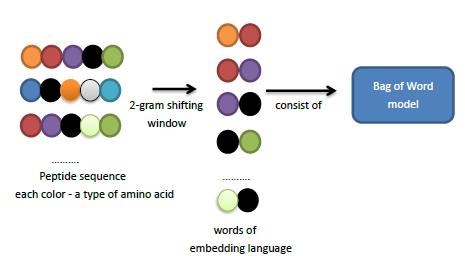
\includegraphics[width=10cm]{./figures/BOW.png}\\
  \caption{Bag of Word}\label{fig:Fig5}
\end{figure}

\todo[inline]{I don't understand the following two paragraphs. Please re-write both of them. Say that to give more meaning to the features, we can include some biological features that are not captured by BOW. The first feature is ... and the second feature is ... . adding these will result in a 402 dimensional feature   }

\noindent
\textcolor{red}{Since the number of the words $w$ in $L$ is directly related to the length of the peptide sequence, the length of the peptide will be used as a feature to characterize the peptide.}\\

\noindent
In addition, knowing that the hydrophobicity is one of the determinative factor of the retention time of the peptide, it is reasonable to include the hydrophobicity of the peptide in the features set too. As the result, we will get the feature matric as fig.\ref{fig:Fig_feature} showed. Each peptide $p_{i}$ is then represented by 402 features as fig.\ref{fig:feature_sub1} and all of them together form the feature matrix as fig.\ref{fig:feature_sub2}.\\

\begin{figure}[h!]
\centering
\subfigure[Feature for each peptide]{
\label{fig:feature_sub1}
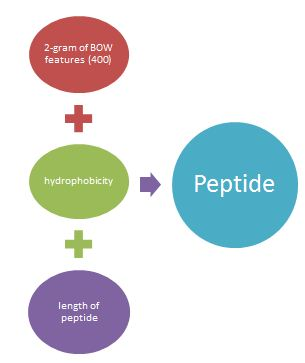
\includegraphics[width=0.4\textwidth]{./figures/feature_structure.jpg}}
\subfigure[Feature matrix for all peptide]{
\label{fig:feature_sub2}
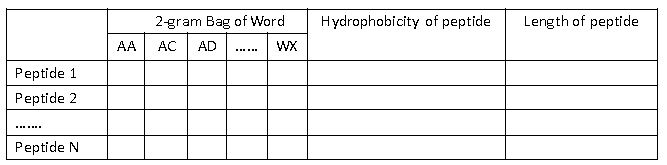
\includegraphics[width=0.8\textwidth]{./figures/feature_mat.jpg}}
\caption{Feature matrix of peptide}
\label{fig:Fig_feature}
\end{figure}


\noindent
The advantages of the Bag-of-Word method are mainly \textcolor{red}{showed}\todo{discussed} in two aspects: complexity and flexibility.\\

\noindent
In terms of complexity, the most popular features that have been used \textcolor{red}{nowadays}\todo{so far} are mainly biochemical features. However, in order to calculate these features, a large amount of time is required. What's worse, some particular facilities are needed to calculate some of them, for example, if we use the structure descriptor as a feature, we need to use some structure analyzer to produce them which is quite expensive and time consuming. Comparing with computing these features, the computational cost of our method is very low. According to \cite{foo17}, the run-time complexity of Bag-of-Word is only $O(|x|+|y|)$ when it is  $O(|x|\cdot |y|)$  for another benchmark method where $x$ and $y$ are the peptide sequences while $|x|$ and $|y|$ are the maximal nonzero dimensions of $\phi_{w}(x)$ and $\phi_{w}(y)$.\\

\noindent
As for the flexibility, since the embedding language $L$ is constituted by the words that are directly and simply extracted from the samples, this method could easily change the language set $L$ for particular context of the task. This property implies a wider applicability in other field of biological research.\\

\section{Gaussian Processes}
\fontsize{12pt}{16pt}\selectfont

By implementing the Bag of Word model, we now have the features to present the peptides in hand. The next step is to establish a nonlinear regression model to find out the relation between the peptide\textcolor{red}{s} and their retention time. In this thesis, we use GP regression model to make \textcolor{red}{the}\todo{this} prediction.\\

\noindent
Gaussian Processes is a supervised machine learning method based on Bayesian theory and statistical learning. In order to understand the theory behind \todo{it} and build an appropriate \textcolor{red}{Gaussian Process}\todo{remove} model, this chapter starts with a brief introduction \textcolor{red}{of}\todo{brief introduction to the ..} the supervised learning method as well as the specification of Standard Bayesian linear Regression. Then we will specify the Gaussian Process in our case along with the detailed mathematical derivation\textcolor{red}{s}. After that, we will specify the concept of multi-kernel functions in Gaussian Process and explain \textcolor{red}{the properties of it}\todo{its properties}. Finally, we will make a comparison between Gaussian Process and the other two methods\textcolor{red}{:}\todo{such as ANN and SVR} ANN and SVR \textcolor{red}{so that we could see the difference of Gaussian Process.}\todo{Remove}

\subsection{Standard Bayesian linear Regression}

Let's first consider a set of \textcolor{red}{input}\todo{observations or samples or data points} $x = \{(x_{i},y_{i}) | i =1,2...n\}$ along with some noise $\epsilon$. In the regression setting, the targets \textcolor{red}{are real values but the observations are with additive noise}\todo{are real values with additive noise.}. We are interested in inferring the relationship between inputs and targets, i.e. the conditional distribution of the targets given the inputs.\\

\noindent
In supervised learning, one way to decide this relationship is using parametric regression which \textcolor{red}{a determines a set of $w$ as the best descriptors of the model between the inputs and outputs}\todo{Re-write}. \textcolor{red}{Now,}\todo{Remove} the problem comes to how to \textcolor{red}{define}\todo{evaluate} if the \todo{trained} model is good enough.\todo{or write : evaluate how the trained model fits the observations.}\\

\todo[inline]{There are two methods for performing this evaluation, loss function and maximum likelihood.}
   
\noindent
\textcolor{red}{To solve this problem, two possible methods have been carried out. Loss Function Method and Maximum Likelihood Method.} The first one is achieved by optimizing the parameters $w$ that minimizing the predefined loss function, such as minimal squared error function (MSE). However, one of the obvious shortages of this method is the over-fitting. To minimize the error of the model, one would increase the complexity of the model that might easily \textcolor{red}{result in the over-fitting problem}\todo{over fit to the training set.}. \todo{This means that} Even though the precision of the model in terms of training data could be high enough, its predictive capacity for unknown data could be really bad and unacceptable. In addition, making a simpler model by ignoring the noise could avoid the over-fitting problem but could also lead to lower accuracy for prediction.\\


\todo[inline]{The main difference between Bayesian regression and loss function is the fact that Bayesian regression considers a prior distribution for $w$, having this distribution prevents the model from over-fitting and forces it to be smooth.}
\noindent
An alternative way to identify the quality of model is Maximum Likelihood, also known as Bayesian regression. The idea of this method is replacing the loss function by the jointly probability distribution with predefined noise (Likelihood function) and search for the parameters $w$ that maximize the likelihood function to build the model.\\

\noindent
Let's consider the dataset $x = \{(x_{i},y_{i}) | i =1,2...n\}$ mentioned before as the input. The Bayesian analysis of the linear regression model can be written as :
\begin{equation} \label{eq:2}
f_{x}=x^{T}w, \quad  y = f_{x}+\epsilon ,
\end{equation}

\noindent
where $x$ is the input vector, $w$ is the parameters(weights) of the input for the linear model. The function value is represented by $ f_{x}$ and a bias (noise) is included. We assume that the $\epsilon$ is independent identically distributed Gaussian noise with zero mean and variance $\sigma_{n} ^{2}$.
\begin{equation} \label{eq:3}
\epsilon \sim N(0, \sigma_{n} ^{2}) ,
\end{equation}

\noindent
The likelihood function, the probability density of the observation given the parameters, will then have the following form:
\begin{equation} \label{eq:4}
p(y|x,w) = \prod_{i=1}^{n}p(y_{i}|x_{i},w) = \prod_{i=1}^{n}\frac{1}{\sqrt{2\pi}\sigma_{n}}exp(-\frac{(y_{i}-x_{i}^{T}w)^{2}}{2\sigma_{n}^{2}})
\end{equation}

\noindent
The idea of Bayesian linear model is mainly based on the posterior distribution computed by Bayes' rule:
\begin{equation} \label{eq:5}
p(w|y,x) = \frac{p(y|x,w)p(w)}{p(y|x)}
\end{equation}

\noindent
To calculate the posterior, we also need a prior over the parameters. The prior is normally considered to represent our prior beliefs over the distribution of the parameters we expect to observe before seeing any data. Therefore, we put a zero mean Gaussian prior with covariance matrix $\Sigma$ on the weights:
\begin{equation} \label{eq:6}
w \sim N(0,\Sigma)
\end{equation}

\noindent
Another essential part is the marginal likelihood function $p(y|x)$. The marginal likelihood,(normalizing constant), gives the likelihood of the output by considering only one specific kind of input and is independent of the other factors. To be specific, the marginal likelihood of expected output here only consider the effect of the input $x$ without taking the effect of the weights $w$ into account. Therefore, it is given by
\begin{equation} \label{eq:7}
p(y|x) = \int p(y|x,w)p(w)dw
\end{equation}

\noindent
By combining the likelihood function in \ref{eq:4} with the prior in \ref{eq:6} and marginal likelihood function in \ref{eq:7}, we could obtain the actual form of the posterior $p(w|x,y)$ in \ref{eq:5}
\begin{equation} \label{eq:8}
p(w|y,x) = \frac{p(y|x,w)p(w)}{p(y|x)} \sim exp(-\frac{1}{2}(w-\bar w)^{T}(\frac{1}{\sigma_{n}^{2}}xx^{T}+\Sigma^{-1})(w-\bar w))
\end{equation}

\noindent
From \ref{eq:8}, it can be seen that the posterior is actually another Gaussian distribution with the new mean and new covariance matrix.\\
\begin{align}\label{eq.9}
    &\bar w= \sigma_{n}^{-2}(\frac{1}{\sigma_{n}^{2}}xx^{T}+\Sigma^{-1})^{-1}xy\notag \\
    &\Sigma_{new} = \frac{1}{\sigma_{n}^{2}}xx^{T}+\Sigma^{-1}
\end{align}

\noindent
For Bayesian linear regression, the prediction is made by all possible parameters along with corresponding posterior probability. Thus, we could conclude the predictive jointly distribution of the output $f_{new}$ of a new data point $x_{new}$ based on the training dataset $x$ along with their weights $w$ and their outputs $y$ as follows :
\begin{align} \label{eq:10}
p(f_{new}|x_{new},y,x) = \int p(f_{new}|x_{new},w)p(w|x,y)dw \notag \\ \sim N(\frac{1}{\sigma_{n}^{2}}x_{new}^{T}(\sigma_{n}^{2}xx^{T}+\Sigma^{-1})^{-1}xy,x_{new}^{T}(\sigma_{n}^{2}xx^{T}+\Sigma^{-1})^{-1}x_{new})
\end{align}



\subsection{Gaussian Processes Regression}

A Gaussian Process regression model inherits the Bayesian theorem and compute the posterior predictive distributions for new test inputs instead of identifying the "best-guess" predictions for them as SVR did.\\

\noindent
A Gaussian Process, a distribution over a set of functions, is fully specified by its mean function and covariance function as \ref{eq:11}
\begin{equation} \label{eq:11}
  f(x) \sim GP(m(x), k(x,x'))
\end{equation}
where the mean function m(x) and the covariance function $k(x, x')$ are:
\begin{equation} \label{eq:12}
  m(x) =  E[(f(x))]
\end{equation}
\begin{equation} \label{eq:13}
k(x,x') = E[(f(x)-m(x))(f(x')-m(x'))]
\end{equation}

\noindent
Normally, for the sake of simplicity,  we will take the mean function to be zero and only consider the effect of covariance function. In fact, the problem of learning in Gaussian Processes is the problem of finding suitable properties for the covariance functions\cite{foo18}.\\

\noindent
Since the Bayesian linear regression model has natural disadvantages in terms of expressiveness and the relationship between our input (peptide sequence) and output (retention time) is barely linear, we take the advantage from Gaussian Processes in terms of dealing with nonlinear problem by utilizing the kernel function. \\

\noindent
The principle of a kernel function is to project the original nonlinear input data into a higher dimensional space where they become linear separable so that the linear model could be implemented directly in that space. The Fig\ref{fig:Fig1} shows the idea of the kernel function\\

\begin{figure}[h!]
  \centering
  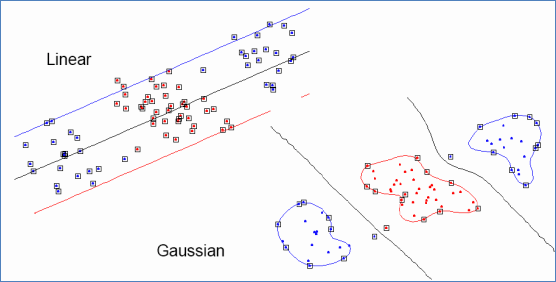
\includegraphics[width=10cm]{./figures/kernel_function.png}\\
  \caption {Projection of data from low-dimensional space into higher dimensional space by Radius Basis Function makes inseparable data separable}\label{fig:Fig1}
\end{figure}

\noindent
To be more specific, the Gaussian Process specifies the covariance function as the kernel function which takes the inner dot product between a pair of random variables. We assume the observations have independent identically distributed Gaussian noise, then the prior of the observations becomes:
\begin{equation}\label{eq:14}
  cov(f(x_{a}),f(x_{b})) = k(x_{a},x_{b})+ \sigma_{n}^{2}\delta_{ab}
\end{equation}

\noindent
where the $k(x_{a},x_{b})$ is a general form of kernel function and $\delta_{ab}$ is a Kronecker delta which is one iff $a\equiv b$ and zero otherwise.\\

\noindent
Then, we could generate the joint distribution of the observations $y$ and the predicted value $f_{new}$ under the prior as
\begin{equation}\label{eq:16}
   \left[
    \begin{array}{c}
     y \\ f_{new}
    \end{array}
   \right] \sim N
   \left(
    \begin{array}{cc}
      0 ,& \left[
           \begin{array}{cc}
            k(x,x)+\sigma_{n}^{2}I & k(x,x_{new})\\
            k(x_{new},x) & k(x_{new},x_{new})\\
           \end{array}
          \right]
    \end{array}
   \right)
\end{equation}



\noindent
Deriving the conditional distribution, we finally arrive at the key predictive equations for Gaussian process regression
\begin{align}\label{eq:17}
   f_{new}|x,y,x_{new} &\sim N(\bar f_{new}, cov(f_{new})), \quad where\\
   \bar f_{new} &= k(x_{new},x)[k(x,x)+\sigma_{n}^{2}I]^{-1}y\\
   cov(f_{new}) &= k(x_{new},x_{new})-k(x_{new},x)[k(x,x)+\sigma_{n}^{2}I]^{-1}k(x,x_{new})
\end{align}

\noindent
These equations give us the corresponding mean value and covariance value of the predictive point which is used to represent the predicted point. A graphical model of Gaussian Processes is can be seen in Fig\ref{fig:Fig2}.

\begin{figure}[h!]
  \centering
  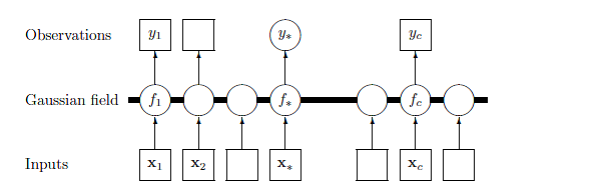
\includegraphics[width=16cm]{./figures/GP_model.png}\\
  \caption {Graphical model for a GP for regression\cite{foo18}.}\label{fig:Fig2}
\end{figure}

\subsection{Kernel Function and Multi-Kernels}

As we could seen from \ref{eq:17}, the accuracy of the estimation of our retention time is highly dependent on the covariance function $k(x_{a},x_{b})$ . In Gaussian Process model, there are several popular covariance functions.\\

\begin{itemize}
  \item Matern covariance:\\
  \begin{equation}\label{eq:kr1}
   k(x_{a},x_{b}) = (1+\frac{\sqrt{3}(x_{a}-x_{b})}{l})exp(-\frac{\sqrt{3}(x_{a}-x_{b})}{l})
  \end{equation}

  \item Linear covariance:\\
  \begin{equation}\label{eq:kr2}
   k(x_{a},x_{b}) = x_{a}\Sigma x_{b}
  \end{equation}

  \item Polynomial covariance:\\
  \begin{equation}\label{eq:kr3}
   k(x_{a},x_{b}) = (x_{a}- x_{b})^{k}
  \end{equation}

  \item Rational quadratic covariance:\\
  \begin{equation}\label{eq:kr4}
   k(x_{a},x_{b}) = (1+\frac{|x_{a}-x_{b}|^{2}}{2\alpha l^{2}})^{-\alpha}
  \end{equation}

  \item RBF covariance:\\
  \begin{equation}\label{eq:kr5}
   k(x_{a},x_{b}) = exp(-\frac{|x_{a}-x_{b}|^{2})}{2l^{2}})
  \end{equation}
\end{itemize}

\noindent
Different covariance function has different properties and generates different similarity measures between pairs of data points. The RBF covariance in \ref{eq:kr5} is the most popular kernel function. In Gaussian process, all these covariance function are weighted by a smoothness factor $\delta_{ab}$ as showed in \ref{eq:14}. This variable together with the parameters in each covariance function are known as the hyperparameters. These hyperparameters will need to be optimized to allow the model to have better performance, This is achieved by maximizing the objective function (marginal log-likelihood function) of GP model. The detail of how to achieve it will be covered in the section of optimization.\\

\noindent
Another interesting thing of these kernel functions is that they could be divided into two types: global kernel function and local kernel function. The RBF kernel function is considered as a typical local kernel while the Polynomial kernel is a global one\cite{foo21}.\\

\noindent
Both types of kernel functions have their own strengths and limitations in different aspects. The local kernel function has strength in terms of approximation but the generalization ability is weak while the global one has stronger generalization ability but weaker approximation capacity.\\

\noindent
We want to take the advantages from the kernel function and eliminate its weakness as much as possible. Therefore, to overcome the weakness of the single kernel function, one simple way is combining those two types of kernel function together as a multi-kernel function, such as the RBF and the Polynomial one.

\begin{equation}\label{eq:222}
  k_{mix} = m*k_{poly} + (1-m)*k_{rbf}  ( 0 \leq m \leq 1)
\end{equation}

\noindent
where $m$ is the weight between two kernel functions. We can see that if $ m = 0$, the multi-kernel is actually a RBF kernel and it is a polynomial kernel when $m = 1$. By combining two kernels as a new one and find a proper weight between them, we could achieve our goal. As for how to find the proper weight factor $m$, we will also explain in the section of optimization. The performance of this multi-kernel function will also be evaluated and compared to the single kernel function later.

\todo[inline]{Properties of Gaussian Process}
\subsection{Property of Gaussian Processes}

As a supervised learning algorithm, the Gaussian Processes is also based on the idea that similar input result in similar outputs or output distributions. But it also have its unique strengths compare with ANN (Backpropagation (BP) algorithm as example) and SVR. \\

\noindent
Since BP algorithm is based on the Empirical risk minimization, it is minimizing the expected error of the model by minimizing the differences between the output of training data and their corresponding true value. This will lead to a serious overfitting problem and poor generalization for new data since it only optimizes the parameters based on training set without considering the test set. Secondly, for a particular BP model, the number of layers of hidden units and the number of units in each layers play an irreplaceable role in ANN algorithm but how to decide these value still remain as a series problem and need to solved. Besides, the BP model adjusted the weights by iteratively calculating the difference between the predicted value and the true ones and giving feedbacks to the system, this principle is in fact similar to the idea of gradient descending. As a result, it will have a low convergence rate and could not guarantee to find the global optima every time.\\

\noindent
As for the SVR, it improves this situation by using structure risk minimization and introducing the penalty coefficient. The structure risk minimization describes the minimization of the sum of the empirical risk and VC confidence which is caused by the complexity of the function space. The VC confidence is related to the amount of training data and could be considered as a reflection of generalization ability of the model. The more training data it has, the smaller the VC confidence will be and the stronger generalization the model will have. These principles could avoid the overfitting problem efficiently and allow the model to have a better generalization capacity. However, the SVR still has many obvious problems such as the choice of the type of kernel function and its parameters and the proper value for the penalty coefficient. In addition, the output of SVR lacks probabilistic meaning.\\

\noindent
The Gaussian Processes is based on the Gaussian distribution and Bayesian theory which implies a solid foundation of probabilistic and statistic. For example, the Gaussian Process not only give the predicted value but also the uncertainty of the prediction. This property makes the prediction easier to interpret and understand. What's more, since Gaussian Processes make the prediction based on the distribution of all data and weaken the contribution of single outlier, it prevents the overfitting problem and gives better generalization capacity than SVR. In addition, in terms of the choice of hyperparameters, the Gaussian Processes is self-adaptive. In other words, the Gaussian Process choose the optimal hyperparameters during its process of training a model while SVR could only choose them by using cross-validation method or based on the pervious experiences. Besides, compared with the BP and SVR model, the number of parameters of Gaussian Processes is quite small which makes the optimization easier to implement.\\

\section{Optimization}
\fontsize{12pt}{16pt}\selectfont

In the Gaussian Process model, the most important part is the covariance function of the model since the Gaussian Process consider it as the kernel function. As we mentioned before, the smoothness factor $\delta_{ab}$ showed in \ref{eq:14} together with the parameters in each covariance function are known as the hyperparameters. These hyperparameters directly determine the properties of the covariance function and further the GP model. Thus, we want to optimize these hyperparameters to get the best combination of these hyperparameters so that we could have a better model for predicting the retention time.\\

\noindent
As for the definition of best combination, we are simply looking for the combination of the hyperparameters that minimizes the value of the objective function. In this case, the objective function is the negative log marginal likelihood of Gaussian Processes as \ref{eq:20}

\begin{equation}\label{eq:20}
  min f(x) =-logp(y|x,\theta)
   =\frac{1}{2}y^{T}(C)^{-1}y+\frac{1}{2}log|C|+\frac{n}{2}log(2\pi)
\end{equation}
where $C =k(x,x)+\sigma_{n}^{2}I_{n}$\\

\noindent
Here, we will implement two different optimization methods based on different principles. The first one is the Conjugate Gradient method and the second one is the Particle Swarm Optimization method. The principle of each method will be explained in detail along with their own strengths and weaknesses towards this case.

\subsection{The Conjugate Gradient}

The conjugate gradient method (CG) is one of the most widely used methods and is developed based on the gradient descending method and Newton Method.\\

\noindent
In CG theory, we have two important assumptions:
\begin{itemize}
  \item Linearity:\\
        the $k_{th}$ search direction $d_{k}$ is the linear combination of all the previous directions.
  \item Conjugation:\\
        all the search direction are conjugated with some positive definitive matrix $A$.
\end{itemize}

\noindent
The first assumption allow us to have the follow equation:

\begin{equation}\label{eq:21}
  d^{k} = -g^{k} + \beta_{k-1}d^{k-1}
\end{equation}
where$g^{k+1}$ is the gradient of the current point and $\beta_{k}$ is some coefficients that need to be calculated. The second assumption is actually used to allow us calculating the $\beta_{k}$\\

\noindent
The process of Conjugate Gradient (CG) method could be described as Fig.\ref{fig:Fig7}
\begin{figure}[h!]
  \centering
  % Requires \usepackage{graphicx}
  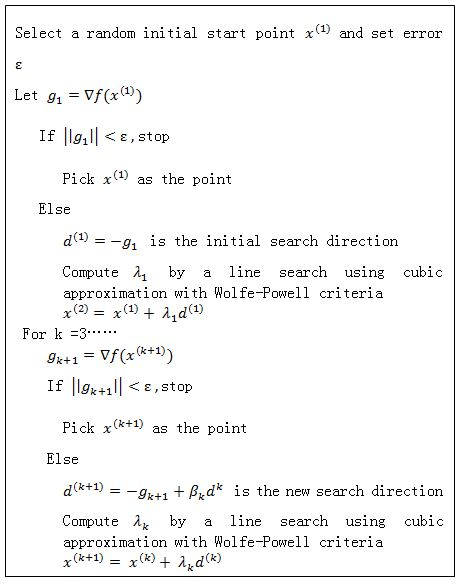
\includegraphics[width=0.6\textwidth]{./figures/CG_algorithm.JPG}\\
  \caption{Conjugate Gradient algorithm}\label{fig:Fig7}
\end{figure}

\noindent
From the algorithm above, we could see the CG method firstly finds a descent direction along which the objective function \ref{eq:20} will be reduced and then computes a step size that determines how far should we move along the direction, aiming at finding a local minimum of the objective function.\\

\noindent
Therefore, the problem could approximately be divided into two parts: Searching the descending direction and determining the step size iteratively. To be more specific, find the proper value for parameters $\beta_{k}$ and $\lambda_{k}$ respectively.\\

\noindent
When it comes to the search direction, due to the second assumption of CG method, we could know that

$$ \beta_{j} =\left\{
\begin{aligned}
  &= 0 \quad j=0....k-1\\
  &\neq 0 \quad j=k
\end{aligned}
\right.
$$

\noindent
Therefore, we are able to compute the $\beta_{k}$ by some methods. In fact, we have many different ways to calculate the parameters $\beta_{k}$ and each of them based on different principles. Here, we implement the Polak-Ribiere method\cite{foo19} that compute the parameter $\beta_{k}$ as \ref{eq:22}.\\

\begin{equation}\label{eq:22}
  \beta_{k} = \frac{g_{k+1}^{T}(g_{k+1}-g_{k})}{g_{k}^{T}g_{k}}
\end{equation}

\noindent
After getting the new search direction $d^{(k+1)}$, the problem comes to define the step size $\lambda_{k}$. Here, we use cubic approximation as \ref{eq:23} to compute the new step size.

\begin{align}\label{eq:23}
   &\lambda_{k} = \lambda_{k-2}-\frac{(-d^{(k-2)}d^{(k-2)})*(\lambda_{k-1}-\lambda_{k-2})^{2}}{(B+\sqrt{(B*B-A*(-d^{(k-2)}d^{(k-2)}))*(\lambda_{k-1}-\lambda_{k-2})})}\notag\\
   &A =6*(f(x_{k-2})-f(x_{k-1}))-3*(-d^{(k-1)}d^{(k-1)}+(-d^{(k-2)}d^{(k-2)}))*(\lambda_{k-1}-\lambda_{k-2})\notag\\
   &B=3*(f(x_{k-1})-f(x_{k-2}))-(2*(-d^{(k-2)}d^{(k-2)})+(-d^{(k-1)}d^{(k-1)}))*(\lambda_{k-1}-\lambda_{k-2})
\end{align}


\noindent
We will then calculate the objective function value $f(x_{k}+a_{k}d_{k})$ and new slope $g_{k+1}^{T}d_{k}$ based on this new step size $\lambda_{k}$ and judge it by using the Wolfe-Powell conditions as \ref{eq:24}

\begin{align}\label{eq:24}
   f(x_{k}+\lambda_{k}d_{k})&\leq f(x_{1})+\lambda_{1} \rho g_{1}^{T}d_{1}\notag\\
   g_{k+1}^{T}d_{k} &\geq \sigma g_{1}^{T}d_{1}  \quad \quad \sigma \in (\rho,1),\quad \rho \in (0,\frac{1}{2})
\end{align}

\noindent
If the current point objective function value and slope fulfill the Wolfe-Powell conditions, we could claim we find the proper step size that is calculated by the cubic extrapolation and stop searching.\\

\noindent
By doing these iteratively, we could minimize the objective function and eventually have the set of hyperparameters $[ w, \sigma , \mu]$ that gives the minimum value of the objective function or fulfills the required accuracy.

\noindent
The CG method is based on the gradient descent and Newton method. It only uses the information provided by the first order derivative which means it does not need any further information and could be easily implemented in many aspects. \\

\noindent
This property also implies that it does not need to compute and store the Hessian Matrix as well as its inverse. As a result, it could reduce the computational cost significantly compared with the Newton method.\\

\noindent
What's more, since the traditional gradient descent method will slow down the searching rate dramatically when it is getting closer to the minimal value, the CG manage to overcome this drawback of the gradient descent by using the conjugation which could speed up the convergence rate. The following plots show the convergence rate of two different methods\\


\begin{figure}[h!]
\centering
\subfigure[Gradient Descent]{
\label{Fig.sub.1}
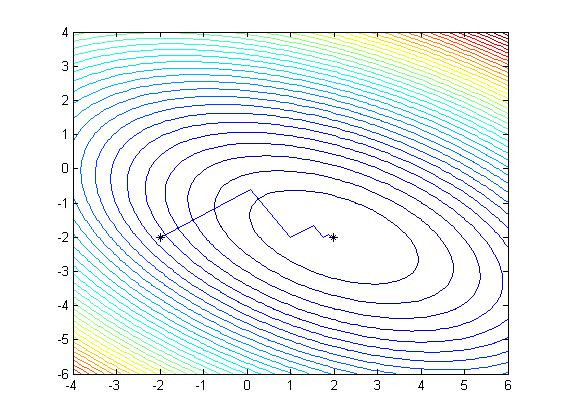
\includegraphics[width=0.4\textwidth]{./figures/Gradient_Descent.jpg}}
\subfigure[Conjugate Gradient]{
\label{fig:sub1}
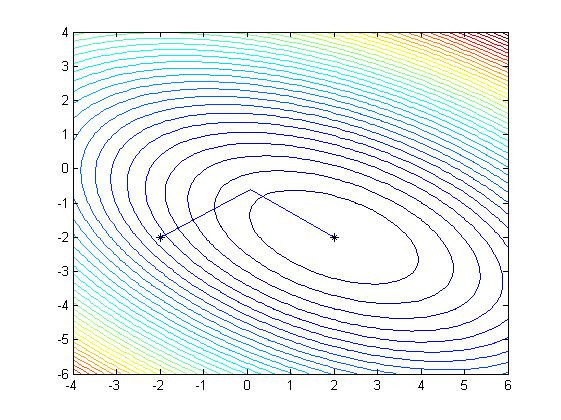
\includegraphics[width=0.4\textwidth]{./figures/CG.jpg}}
\caption{Comparison of convergence rate}
\label{fig:sub2}
\end{figure}


\subsection{The Particle Swarm Optimization}

The Particle Swarm Optimization (PSO) method is one of the new iterative methods for problem optimization. It improves the solution by iteratively searching for the best result in current circumstance. \\

\noindent
Initially, we have a branch of separated particles that represent the potential solution by their position, a group of the hyperparameters in our case. And for each parameter in the one particle, we assign different velocity for them. In each iteration, the particle updates its position simply by its velocity of each parameter. Then we use these parameter to calculate the model and evaluate the result by some predefined loss functions. After that, we record the best position for each particle(local optimal value) as well as the best position in the whole search space(global optimal value).\\

\noindent
The smart part of this method is the update of the velocity of each particle. The individual velocity for each particle is influenced not only by its local best known position (local optimal value) but also the best known positions in the search-space (global optimal value), which are updated as better positions are found by other particles. This is expected to move the swarm toward the best solution.\\

\noindent
In the end, the iteration will be terminated by some criterion, such as the maximal number of iterations or a solution that gives the adequate loss function value is found. The following Fig. \ref{fig:Fig8} shows the basic algorithm of Particle Swarm Optimization \\

\begin{figure}[h!]
  \centering
  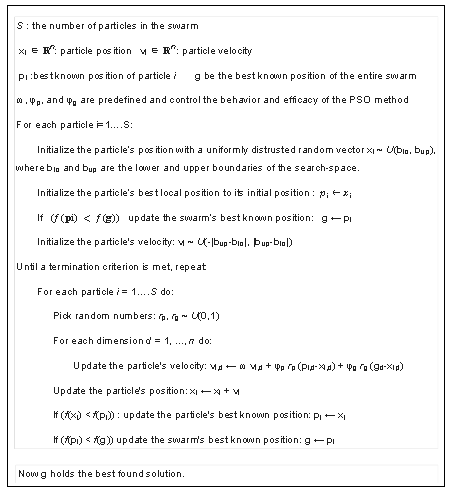
\includegraphics[width=0.9\textwidth]{./figures/PSO.png}\\
  \caption{Particle Swarm Optimization}\label{fig:Fig8}
\end{figure}

\noindent
PSO is a heuristic search algorithm based on swarm intelligence since it makes no assumptions about the problem being optimized and can search very large spaces. Therefore, PSO can also be used on optimization problems that are partially irregular, noisy, change over time, etc. What's more, since it uses swarm intelligence which means each of the particle is related to the others and the final result is depended on the contribution of all particles, the robustness of system is strong and will not be be dramatically influenced by some outliers. In addition, its strengths in terms of convergence, global search capacity and practicability also make it one of the most popular optimization algorithm in the world. \\

\section{Summarize of the Chapter}

After optimizing the hyperparameters, the GP regression model is ready to predict the peptide's retention time. The general process of this chapter could be illustrated as the fig.\ref{fig:framework} and the performance of the GP model will be showed in the next chapter.\\

\begin{figure}[h!]
  \centering
  % Requires \usepackage{graphicx}
  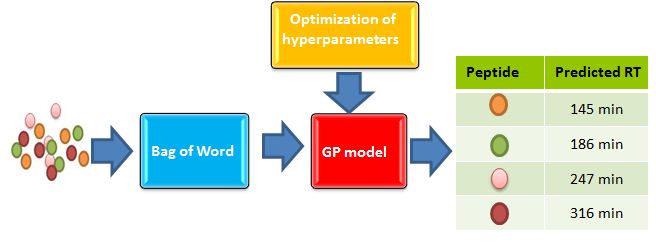
\includegraphics[width=1\textwidth]{./figures/workflow.jpg}\\
  \caption{The general process of predicting peptide's retention time}\label{fig:framework}
\end{figure}



\chapter{Results and Evaluation}
\fontsize{12pt}{16pt}\selectfont

In this section, we report the experiments in order to compare the GP regression model with other prediction models and discuss their performance. We are interested in whether the GP model leads to a better predictive performance than the other models as well as its strengths and weakness compared with other models.\\

\noindent
To get a better impression of the performance, we will firstly investigate the importance of kernel functions. To be specific, we will compare the GP model with single kernel to the one with multiple kernels. Further, we will investigate the importance of optimization. In another word, we will compare the results before and after optimization for GP model. After this comparison, we will evaluate the performance of different optimization methods, PSO and CG method specifically. All these models will be tested in two different set of features respectively so that we could make a comparison between different kind of features. The first kind of feature is the feature created by Bag of Word method: we simply call it $BOW feature$, and the second one is the features used for prediction in the state-of-art model Elude: we call it $Elude feature$.\cite{foo5}\\

\noindent
In the end of this part, we will make a comparison between different kinds of state-of-art retention time predictors including Elude, BioLCCC (an on-line retention time predictor)\cite{foo24},SSRC and our GP model. These models will be tested by the peptide we use for the GP model and evaluated by the same criteria as show below. \\

\noindent
Before introducing the experimental setup, we will first introduce some main concepts which we will use for the result evaluation later: Pearson Correlation Coefficient and minimal time window.
\begin{itemize}
  \item Pearson Correlation Coefficient:\\
        In statistic theory, Pearson correlation coefficient is used to identify the linear correlation between two variables $X$ and $Y$. The formula is as follow:
\begin{equation}\label{eq:25}
   \rho = Cor(X, Y) = \frac{Cov(X,Y)}{\sqrt{Var(X)Var(Y)}}
\end{equation}
        The value of Pearson Correlation Coefficient is between -1 and 1. A value of 1 (or -1)implies that a linear equation describes the relationship between X and Y perfectly, the sign implies whether the relationship is positive or negative. A value of 0 implies that there is no linear correlation between the variables. The closer the value is to 1, the stronger the linear relation they have, otherwise, the weaker the relation they have.\\
  \item Minimal Time Window:\\
        The minimal time window is a time window including the
        deviations between observed and predicted retention times for 95\% of the peptides ($\Delta t95\%$). Given the time window, we could know the expected range of observing time in advance and thus enhanced paralleling generating ability of the retention time of peptide. In this case, the minimal time window will be showed as ratio of total time instead of a absolute value. The total time is defined as the time interval between the smallest observed retention time and largest one. The smaller the time window is, the more peptide we could generate at the same time.
  \item Computational Cost:\\
        The computational cost is a parameter reflects the efficiency of a model. A model with too large computational cost should be considered as a bad model since it is hard to implement and reproduce. The computational cost in this thesis stands for the total running time from importing raw peptide data to getting the predicted retention time of the peptide.

\end{itemize}

\noindent
In this thesis, the top priority is given to minimize the minimal time window since we want to be able to generate as many peptide as possible and improve the parallelized processing capacity. Therefore, even if the Pearson coefficient coefficient of model A is sightly better than model B, we still claim the model B has better performance than A when the minimal time window of model B is smaller than A.

\section{Experimental Setup}
\noindent
The experiment is tested on a 64-bit Ubuntu computer and run by Matlab R2014a. To build the Gaussian Process model, we need to install the software package called GPML which is written by Carl Edward Rasmussen and Hannes Nickisch.\cite{foo18} In addition, to benchmark the GP model, we also need the SVR software packages libsvm \cite{foo20}.\\

\noindent
The experimental data we use in this thesis is a set of 15933 peptides generated from the laboratory as \ref{fig:data}. We separate them into training set and testing set respectively. The training set contains 12747 peptides while the testing set has 3186 peptides.\\

\begin{figure}[h!]
  \centering
  % Requires \usepackage{graphicx}
  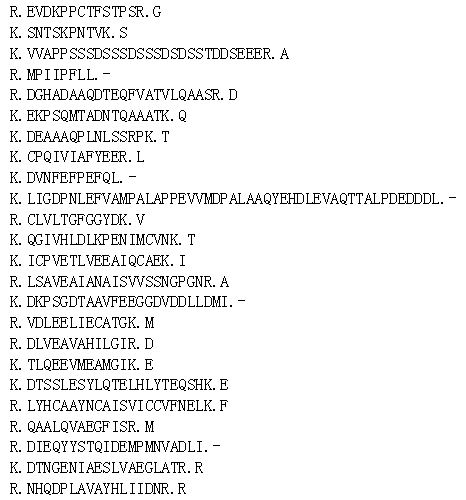
\includegraphics[width=0.4\textwidth]{./figures/data.jpg}\\
  \caption{a subset of experimental peptide sequence}\label{fig:data}
\end{figure}

\section{Experimental Results}

\begin{figure}[h]
\centering
\subfigure[Bag of Word feature with RBF kernel]{
\label{Fig.sub.1}
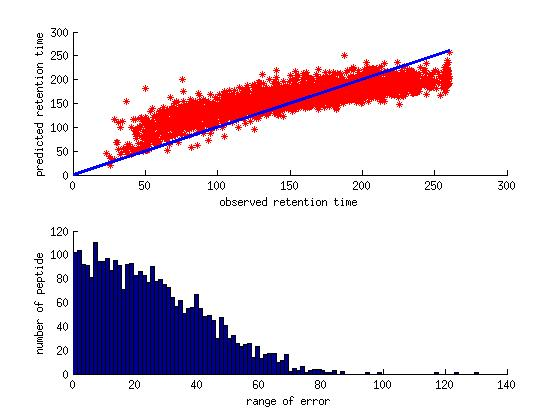
\includegraphics[width=0.4\textwidth]{./figures/original_without_opt_usingbow.jpg}}
\subfigure[Bag of Word feature with RBF+Poly kernel]{
\label{Fig.sub.2}
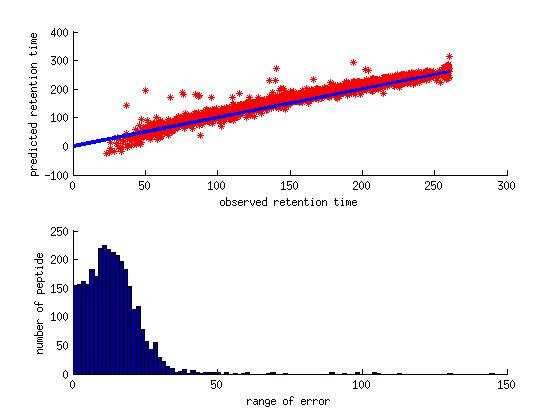
\includegraphics[width=0.4\textwidth]{./figures/original_without_opt_bowfeature_multikernel.jpg}}
\caption{Comparison of performance based on different kernels} \label{fig:Fig9}
\end{figure}

\noindent
The Gaussian Processes model is firstly built by $BOW feature$. The Fig.\ref{fig:Fig9} shows the performance of the GP model based on different kernel function. The left one is simply using RBF kernel while the right one is using a multiple kernel that consist of RBF and Poly kernel function. The blue line in the plot represents the ideal result of the correlation coefficient and the red one is the true results from the experiment.\\

\noindent
For each subplot, the top plot shows the correlation between the predicted retention time and the real retention time and tells how linear they are related to each other. The histogram in the bottom shows the the distribution of the deviation between the predicted retention time and the real one. \\

\noindent
As benchmark, we also test the model by using $Elude feature$. The fig.\ref{fig:Fig10} gives us the performance of the model based on this feature set.\\

\begin{figure}[h!]
\centering
\subfigure[Elude feature with RBF kernel]{
\label{fig:sub1}
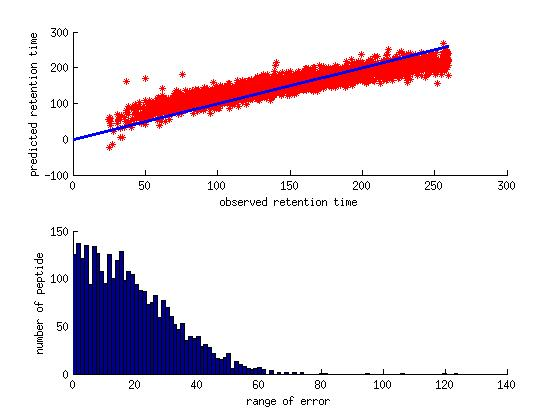
\includegraphics[width=0.4\textwidth]{./figures/original_without_opt.jpg}}
\subfigure[Elude feature with RBF+Poly kernel]{
\label{Fig.sub.2}
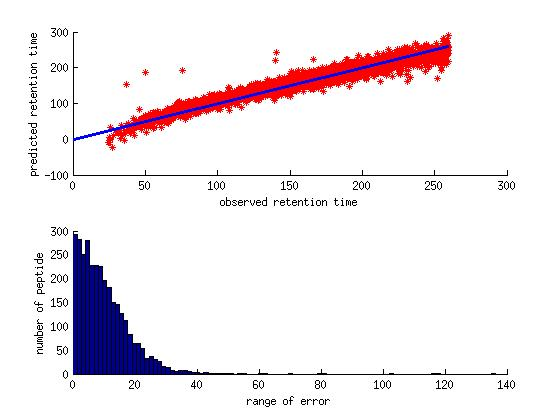
\includegraphics[width=0.4\textwidth]{./figures/Lumi_RBF+poly_without_opt_GP.jpg}}
\caption{Comparison of performance based on different kernel with Luminita's feature}
\label{fig:Fig10}
\end{figure}

\noindent
The Table.\ref{table1} shows detail information in terms of the Pearson Correlation Coefficient and the minimal time window of them. The left number is the Person Coefficient and the right one is the corresponding minimal time window.\\

\begin{table}[h]
\normalsize
\centering
\begin{tabular}{l|cc|cc}
         & \multicolumn{2}{c|}{RBF kernel} & \multicolumn{2}{c}{RBF + Poly kernel}\\
         & $\rho$ & $\Delta_{t95\%}$ & $\rho$ & $\Delta_{t95\%}$ \\
        \hline
         BOW feature & 0.8506 & 0.5080 &  0.9674 &  0.2474\\
        \hline
         Elude feature  & 0.9213 & 0.3912 &  0.9737 & 0.2052\\
        \hline
\end{tabular}
\caption{Comparison between Single kernel and multi-kernel}
\label{table1}
\end{table}

\noindent
As we can see from the figures, the multi-kernel gives better performance than a single kernel in general. The multi-kernel function helps GP model to improve the correlation coefficient in both cases. The scatter plots in both cases become narrower and closer to the ideal blue line.\\

\noindent
More importantly, it also reduces the minimal time window dramatically, from 0.5080 to 0.2474 and 0.3912 to 0.2052 for $BOW feature$ and $Elude feature$ respectively. This also implies that the multi-kernel makes the prediction more precisely and narrow down the deviations between observed and predicted retention times.\\

\noindent
After comparing the Gaussian Process with single kernel and multi-kernel, we will now investigate the effect of optimization. In this case, we only perform Particle Swarm Optimization method as an example. The following plots show the results\\


\begin{figure}[h!]
\centering
\subfigure[BOW feature with GP model]{
\label{fig:sub1}
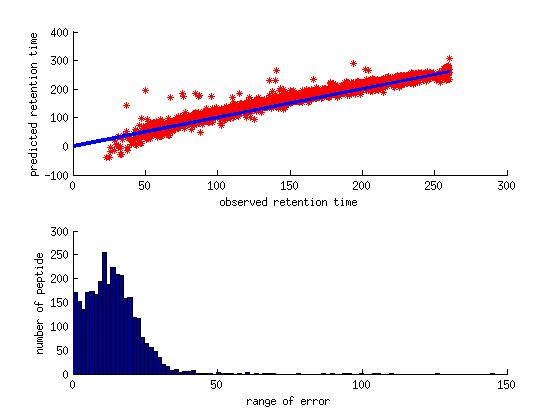
\includegraphics[width=0.4\textwidth]{./figures/PSO_fig1_bow.jpg}}
\subfigure[Elude feature with GP model]{
\label{Fig.sub.2}
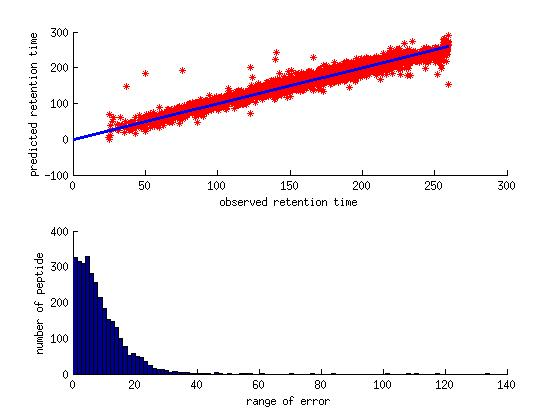
\includegraphics[width=0.4\textwidth]{./figures/PSO_fig1_Lumi.jpg}}
\caption{Performance of the feature based on Gaussian Process model after PSO optimization}
\label{fig:Fig14}
\end{figure}

\begin{table}[h]
\normalsize
\centering
\begin{tabular}{p{1cm}|p{2cm}|p{3.5cm}|p{3.5cm}}
\multicolumn{2}{c|}{} & Before Optimization & After Optimization \\
\hline
\multirow{2}{*}{GP} & BOW  & 0.9674 \quad 0.2474 & 0.9753 \quad 0.2379 \\
\cline{2-4}
 & Elude & 0.9737 \quad 0.2052 & 0.9741 \quad 0.1944 \\
\hline
\end{tabular}
\caption{Comparison of performance before and after PSO for GP}
\label{table2}
\end{table}

\noindent
From Table.\ref{table2}, we could tell that the PSO optimization is useful and have improved the prediction result. Although the difference is only $0.01$, it is about 1 min of the deviations between observed and predicted retention times.\\

\noindent
However, we could not deny that the optimization method in this case does not make a significant difference to the prediction results. The potential explanations for this phenomenon could be as follows: \\

\noindent
First of all, the initial parameters for the model is too prefect and the better solution that the optimization method have found could not make a significant improvements. Secondly, the PSO optimization method itself is not appropriate and could not find some much better solution. Thirdly, it has not found the optimal combination for the hyperparameters this time due to the fact that the PSO method does not guarantee to find the optimal solution every time.\\

\noindent
Among all these probabilities, the third second and the third explanations are probably the reasons for this phenomenon. To investigate more about the reasons, we will now try to compare the PSO method with another optimization method, Conjugate Gradient method, to see if our explanations are correct.\\

\noindent
The following plots show the experimental results of different optimization methods.\\

\begin{figure}[h!]
\centering
\subfigure[BOW feature with PSO]{
\label{fig:sub1}
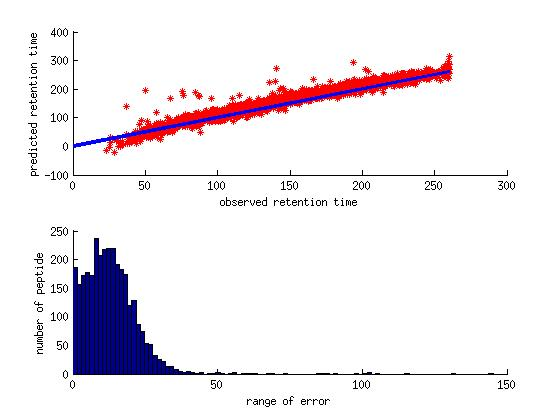
\includegraphics[width=0.4\textwidth]{./figures/PSO_fig1_BOW_mk.jpg}}
\subfigure[BOW feature with CG]{
\label{Fig.sub.2}
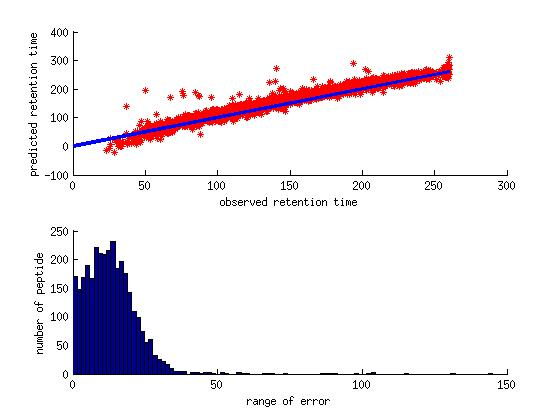
\includegraphics[width=0.4\textwidth]{./figures/CG_fig1_BOW_50times_iter.jpg}}
\caption{Performance of the BOW feature based on different optimization method}
\label{fig:Fig15}
\end{figure}

\begin{figure}[h!]
\centering
\subfigure[Elude feature with PSO]{
\label{fig:sub1}
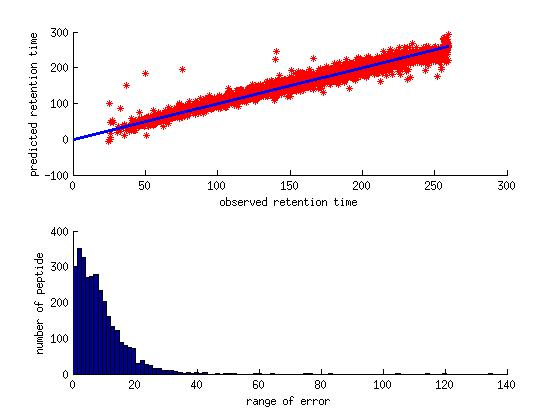
\includegraphics[width=0.4\textwidth]{./figures/PSO_fig1_Lumi_mk.jpg}}
\subfigure[Elude feature with CG]{
\label{Fig.sub.2}
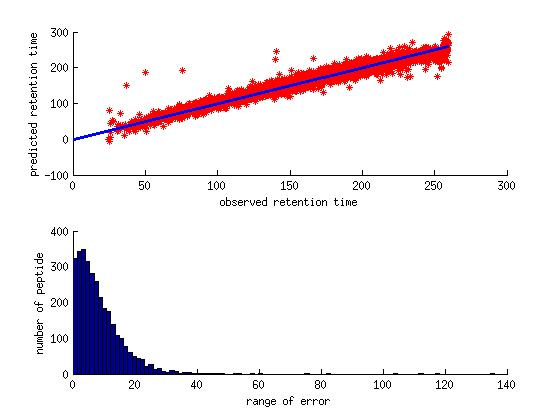
\includegraphics[width=0.4\textwidth]{./figures/CG_fig1_Lumi_50times_iter.jpg}}
\caption{Performance of the Elude feature based on different optimization method}
\label{fig:Fig16}
\end{figure}

\noindent
As we can see from fig.\ref{fig:Fig15} and fig.\ref{fig:Fig16} , these two methods have similar performance in this case. However, when we look at the details of the comparison of these two optimization in Table.\ref{table3}, we could see that the CG method actually gives better performance than the PSO method. If we combine this with the Table.\ref{table2}, we could tell that the CG method is more appropriate than PSO method in this case. It reduces the $\Delta_{t95\%}$ of $Elude feature$ from $0.2052$ to $0.1908$ and the one of $BOW feature$ from $0.2474$ to $0.2326$. Another interesting thing to see is that the result of PSO method in two tables are different and the result in Table.\ref{table3} is better than table.\ref{table2}. This is exactly what we have guessed that the PSO does not guarantee to find the optimal solution every time.\\

\begin{table}[h!]
\centering
\begin{tabular}{l|cc|cc}
   & \multicolumn{2}{c|}{Particle Swarm Optimization} & \multicolumn{2}{c}{Conjugate Gradient}\\
   & $\rho$ & $\Delta_{t95\%}$ & $\rho$ & $\Delta_{t95\%}$ \\
\hline
 BOW  & 0.9740 & 0.2329 & 0.9760 & 0.2326 \\
\hline
 Elude & 0.9741 & 0.1944 & 0.9762 & 0.1908 \\
\hline
\end{tabular}
\caption{Comparison of performance of GP based on PSO and CG optimization}
\label{table3}
\end{table}

\noindent
About the optimization methods, apart from having a impression of the general performance, we would also like to investigate the influence of some parameters for the prediction, such as the number of evaluating function, the number of generation, the number of particles and the changing trend of each particle during the evolution.\\

\begin{figure}[h!]
\centering
\subfigure[BOW feature with CG]{
\label{fig:sub1}
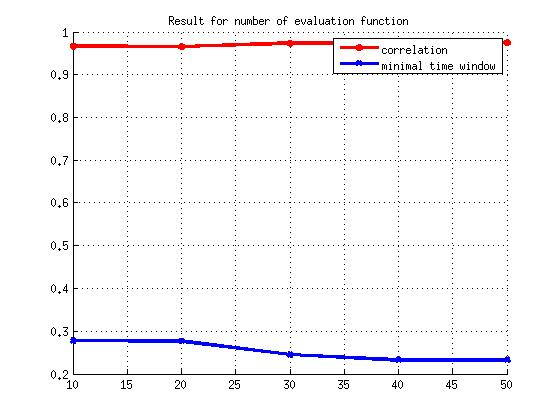
\includegraphics[width=0.4\textwidth]{./figures/CG_fig2_bow_cp.jpg}}
\subfigure[Elude feature with CG]{
\label{Fig.sub.2}
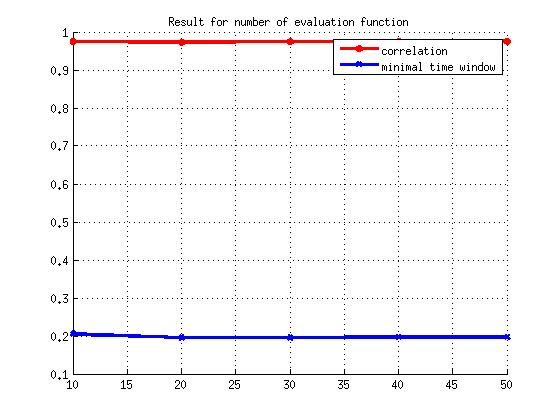
\includegraphics[width=0.4\textwidth]{./figures/CG_fig2_lumi_cp.jpg}}
\caption{Comparison of different number of evaluating functions}
\label{fig:Fig17}
\end{figure}

\noindent
The fig.\ref{fig:Fig17} show the effect of different number of evaluating function in CG method based on different features. As we can see, increasing the number of evaluating function results in better performance in terms of correlation coefficient and minimal time window. However, when the number of evaluating function reaches to the level of 30 and above, the difference becomes small and can be ignored. These plots implies that we could set the number of evaluating function around 30 and no need to worry about not getting better prediction result. \\

\noindent
Following this, we will now try to find out the influence of the number of generation in PSO methods.\\

\begin{figure}[h!]
\centering
\subfigure[BOW feature with 5 generation]{
\label{fig:sub1}
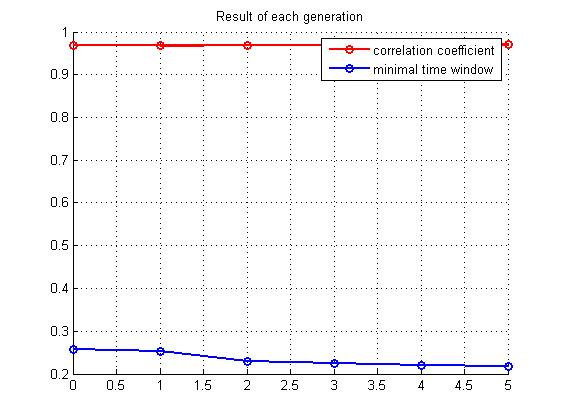
\includegraphics[width=0.5\textwidth]{./figures/PSO_bow_5generation.jpg}}
\subfigure[BOW feature with 30 generation]{
\label{Fig.sub.2}
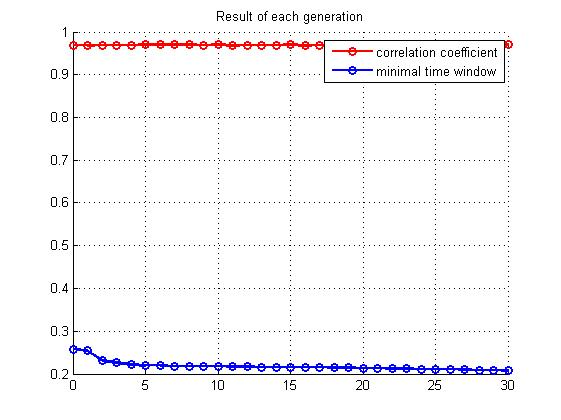
\includegraphics[width=0.5\textwidth]{./figures/PSO_fig2_BOW_mk_30generation.jpg}}
\caption{Comparison of different number of generation}
\label{fig:Fig18}
\end{figure}

\noindent
The fig.\ref{fig:Fig18} shows that the number of generation actually have slightly influence on the prediction. The top one traces the changing trend of correlation coefficient and minimal time window during 5 generation and in the bottom one, we increase the number of generation to 30 to make a comparison. Each dot in the plots represent the prediction result of that generation.\\

\begin{figure}[h!]
\centering
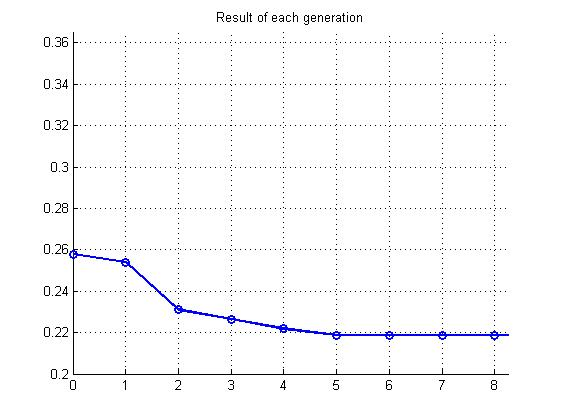
\includegraphics[width=0.5\textwidth]{./figures/zoom_in_30generation.jpg}
\caption{Detail changes of 30 generation}
\label{fig:Fig19}
\end{figure}

\noindent
The detail could be seen from fig.\ref{fig:Fig19}. The optimization has reduced the minimal time window from around 22\% to around 19\% in the second generation of evolution. Due to the fact that the prediction after the first few generation is already really good, the impact of increasing the number of generation seems to be ignorable. The Table.\ref{table4} shows the detail information based on different number of generation.\\

\noindent
Another problem comes along with increasing the number of the generation is that the computational cost becomes increasingly large. For example, the computational cost of a GP model with $BOW feature$ using 5 generation PSO method is $1701 sec$ while the one using 30 generation PSO is $5661 sec$ which is 3 times as much as before. The situation becomes even worse when the number of the features increase. Therefore, we could simply set the default number of generation around 5. \\

\begin{table}[h!]
\centering
\begin{tabular}{l|cc|cc}
   & \multicolumn{2}{c|}{5 generation} & \multicolumn{2}{c}{30 generation}\\
   & $\rho$ & $\Delta_{t95\%}$ & $\rho$ & $\Delta_{t95\%}$ \\
\hline
 BOW  & 0.9740 & 0.2329 & 0.9760 & 0.2325 \\
\hline
 Elude & 0.9741 & 0.1944 & 0.9762 & 0.1933 \\
\hline
\end{tabular}
\caption{Best performance of GP model based on PSO with different number of generation}
\label{table4}
\end{table}

\noindent
Now, we will take a look at the effect of different number of particles and each particle's evolution trend in terms of correlation coefficient and minimal time window during each generation.\\

\begin{figure}[h!]
\centering
\subfigure[Trend of correlation coefficient of each particle]{
\label{Fig.sub.201}
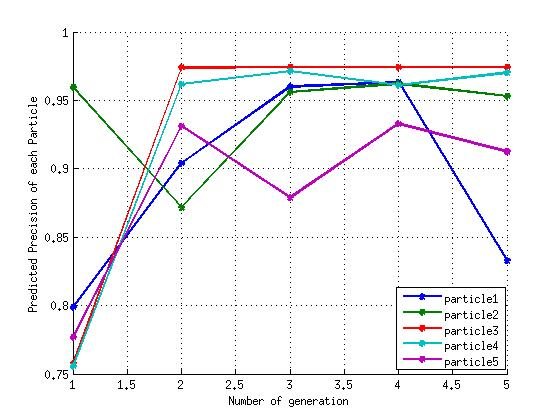
\includegraphics[width=0.4\textwidth]{./figures/PSO_fig3_Lumi.jpg}}
\subfigure[Trend of minimal time window of each particle ]{
\label{Fig.sub.202}
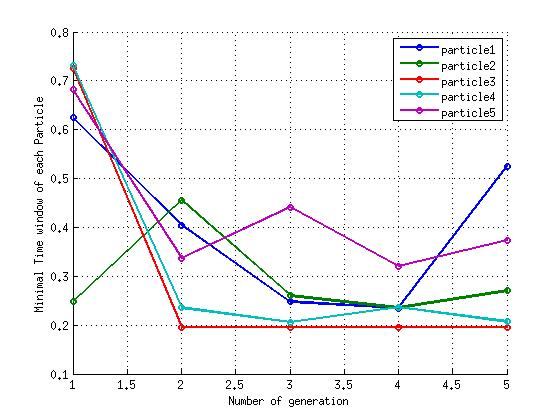
\includegraphics[width=0.4\textwidth]{./figures/PSO_fig4_Lumi.jpg}}
\caption{The evolution trend of each particle during 5 generations with 5 particles}
\label{fig:Fig20}
\end{figure}

\begin{figure}[h!]
\centering
\subfigure[Trend of correlation coefficient of each particle]{
\label{Fig.sub.211}
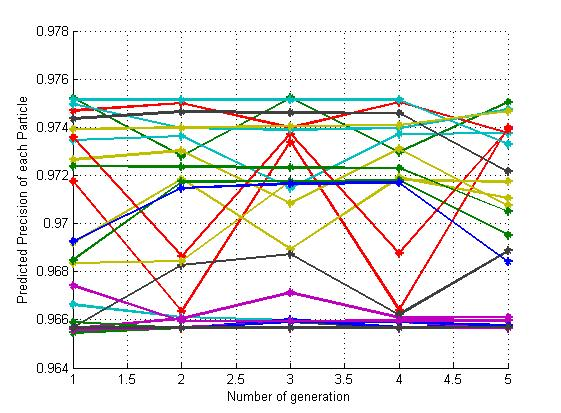
\includegraphics[width=0.4\textwidth]{./figures/changing_trend_of_coef_30par.jpg}}
\subfigure[Trend of minimal time window of each particle ]{
\label{Fig.sub.212}
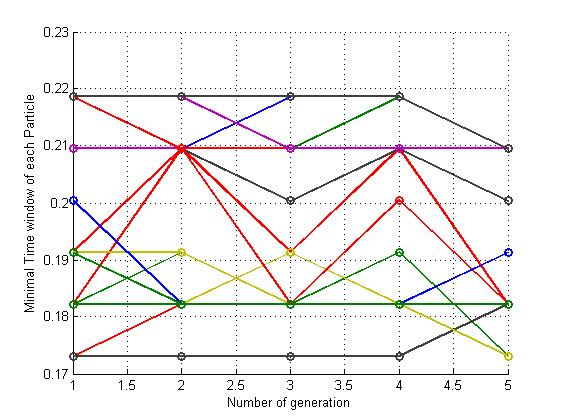
\includegraphics[width=0.4\textwidth]{./figures/changing_trend_of_mtw_30par.jpg}}
\caption{The evolution trend of each particle during 5 generations with 30 particles}
\label{fig:Fig21}
\end{figure}

\noindent
As the Fig.\ref{Fig.sub.201} and Fig.\ref{Fig.sub.202} showed, the trend of all the particles in both cases are going towards the better situation and have influenced each other which totally follows the principle of PSO method. As comparison, we also display the results of using 30 particles instead of 5 particles. These plots show that each individual particle's evolution is basically random but most of the particles are going towards the same direction when seeing the main trend from a bigger picture. Besides, it can be seen from Table.\ref{table5}that increasing the number of particles do not contribute much to the improvement of both accuracy and minimal time window. One interesting thing is that we could also see the trend becomes more flat and stable after the third generation. This is also support evidence for the conclusion we draw form Fig.\ref{fig:Fig19} about the proper number of generation.\\

\begin{table}[h!]
\normalsize
\centering
\begin{tabular}{l|cc|cc}
   & \multicolumn{2}{c|}{5 particles of PSO} & \multicolumn{2}{c}{30 particles of PSO}\\
   & $\rho$ & $\Delta_{t95\%}$ & $\rho$ & $\Delta_{t95\%}$ \\
\hline
 BOW  & 0.9740 & 0.2329 & 0.9747 & 0.1731 \\
\hline
 Elude & 0.9741 & 0.1944 & 0.9757 & 0.1537 \\
\hline
\end{tabular}
\caption{Comparison of performance based on different number of particles}
\label{table5}
\end{table}

\noindent
In the end, as benchmark, we will summarize the performance of other popular retention time prediction models and compare them with our GP model in terms of correlation coefficient$\rho$ , minimal time window($\Delta_{t95\%}$) and computational cost. The Table.\ref{table6} shows the result of different models.\\

\begin{table}[h!]
\normalsize
\centering
\begin{tabular}{l|c|c|c|c}
   & GP Model & Elude Model & SSRC  & BioLCCC \\
\hline
 Pearson Correlation Coefficient($\rho$) & 0.9757 & 0.9879 & 0.9064 & 0.9153  \\
\hline
 Minimal Time Window($\Delta_{t95\%}$) & 0.1908 & 0.1651 & 0.4028 & 0.3750 \\
\hline
 Computational Cost & 1731 sec & 16323 sec & \ & \ \\
\hline
\end{tabular}
\caption{Comparison of performance based on different number of particles}
\label{table6}
\end{table}

\noindent
The last two columns are empty because we do not know how long it takes to train the model for prediction.\\

\noindent
As we can seen form Table.\ref{table6}, our GP model gives much better performance than SSRC and BioLCCC. Our model successfully reduce the $\Delta_{t95\%}$ to a level of $0.1908$ while the BioLCCC only gives $0.3750$ and result of SSRC is $0.4028$. That means our model reduces almost 20 mins of the time window which enhance the parallelized processing ability dramatically. In addition, the $\rho$ of our GP model is also higher than the SSRC and BioLCCC which means our prediction is more precise than the other two methods.\\

\noindent
What's more, our GP model gives similar performance as Elude which is considered to be the most popular and best model so far. Although the Elude gives better performance in both correlation coefficient and minimal time window, the computational cost of Elude is much higher than our GP model. In big data analysis, such high computational cost could be a very serious problem and we should make a balance between the accuracy and the efficiency. Considering that the computational cost of Elude is almost 10 times as our GP model, the $\rho$ and $\Delta_{t95\%}$ of our GP model are still good enough and our model has stronger practical ability than Elude.

\chapter{Discussion and Conclusion}
\fontsize{12pt}{16pt}\selectfont

\section{Limitation and Discussion}

As we discussed in the previous chapter, GP outperforms most other models. However, there are still some limitations \textcolor{red}{of}\todo{on} this model that needs to be improved.

\todo[inline]{Maybe : However, in this chapter we will discuss several limitations of this model. Solving these limitations can have a significant impact on the accuracy of our method.}

\subsection{Model limitation}

One of the main limitation is the computational cost of Gaussian Process model. Although the computational cost of our GP model is better than Elude, it is still a main problem due to the fact that the Gaussian Process Regression model is a non-parametric model. For training part, the hyperparameters are obtained by optimizing the likelihood function. Therefore, we need to compute the inverse of covariance function $K_{n} + \sigma_{n}^{2}I_{n}$  which makes the computational cost of the model to a level of  $O(n^{3}*p)$ where $p$ is the times of gradient computation. As for the prediction part, the computational cost for each data is $O(n^{2})$. When dealing a large amount of data, this drawback could become more serious and do harm to the implementation.\\

\noindent
Another limitation of the GP model is the assumption of the  \textit{Gaussian Noise} which means the noise needs to fulfill the Gaussian distribution. This assumption makes the GP model easier when calculating the matrix. However, the noise is actually not a \textit{Gaussian Noise} in some cases and this assumption will therefore influence the prediction and leads to worse results.\\

\subsection{Feature limitation}


As for the features, the main limitation is the lack of information for our features. This means the \textit{BOW features} do not have significant biological meaning.  This limitation is reflected by the fact that the \textit{Elude features} performs better than the \textit{BOW features} in general. \\

\noindent
However, on one hand, providing features with more information means the prediction are more likely to be precisely. On the other hand, compared to \textit{BOW features}, the \textit{Elude features} requires more time to be calculated. More importantly, the performance of these two features is actually not very different. This means that the features that are suitable for this task are still unknown and finding those features will require further investigation.\\


\subsection{Optimization limitation}

\noindent
Like most evolutionary algorithms, PSO usually requires a large number of fitness evaluations to obtain a sufficiently good solution. This poses an obstacle for applying PSO to computationally expensive problems.\\

\noindent
Besides, as all other heuristic algorithms, PSO do not guarantee an optimal solution is ever found. In fact, the optimized result could be slightly different from time to time but always has the same trend. More specifically, PSO does not use the gradient of the problem being optimized, which means PSO does not require that the optimization problem be differentiable as is required by classic optimization methods such as gradient descent and quasi-newton methods. As a result, it might find the local optimal value instead of the optimal value in the whole search space and consider it as the "global optimal value" due to the its convergence. \\

\noindent
To overcome the shortages of the PSO method, a number of different methods based on the original PSO have been carried out, such as Gray-PSO, Chaos-PSO. Each of these methods has combined PSO with some other method so that it could overcome the problem of the original PSO and have their own advantages when dealing with some specific tasks. \\

\noindent
As for the CG method, one of the most limitation of the CG method is its dependency on the initial point which would have a great influence on the final result. Due to this limitation, the CG method could not ensure to converge to the minimum value in the whole search space.\\

\noindent
To overcome this, there are many variations of CG. They could improve the performance of the original CG method when dealing with some specific tasks but they still have their drawbacks as well. \\

\section{Conclusion}

\noindent
In this thesis, GP model has been proposed for the prediction of peptide retention time has been proposed and tested in different datasets. The importance of kernel function has been investigated and comparison has been made between single kernel function and multi-kernel function. The multi-kernel function combines the strengths of two kernel functions and improves the accuracy of the prediction results significantly.\\

\noindent
Secondly, a new method of feature selection has been tested in this case. The feasibility of these features has been proved and their performance is almost as good as the biochemical features. Although the performance of these less-biochemical features are still slightly worse than the biochemical features due to the fact of lacking information, the efficiency of generating them and the flexibility of these features still imply the unique and powerful advantages.\\

\noindent
In addition, two optimization methods have been implemented and compared with each other. Although, we only utilize the original version of them, they still make a significant impact on the experimental results.\\

\noindent
Finally, the GP model was also compared with the other state-of-art prediction methods. The GP model has better performance than most of them in terms of the minimal time window ($\Delta_{t95\$}$) and correlation coefficient ($\rho$). Even compared with the best predicted model Elude, the predicted result of our model is still similar.\\

\noindent
This implies our model in general has stronger processing capacity and could identify more peptide than the other models at the same time. Besides, the computational efficiency of our model is much higher than Elude model when having similar identification capacity. This is a significant and useful quality since a lot of biochemical experiments contain large amount of data that need to be processed.\\


\section{Future Work}


As we have analyzed before, one of the most important limitations of GP model is the computational cost. It is quite hard to overcome this problem since the Gaussian Process is non-parametric model. In the last 20 years, many new methods have been proposed to solve this problem. Tresp in \cite{foo22} proposes a Bayesian committee machine(BCM) method and Snelson in \cite{foo23} suggest a method based on sparse Gaussian Process using pseudo-input to enhance the computational efficiency. Therefore, one potential work in the future is to replace the original Gaussian Process with these new methods to investigate their performance. What's more, one could even implement some new machine learning methods, such as deep learning to address this problem and test their performance.\\

\noindent
Another potential direction to go on is the feature selection method. Currently, we only test two different kinds of features separately and both of them give similar performance. So a alternative way to continue is try to combine different types of feature together as new multi-features and investigate their performance.\\

\noindent
One more interesting thing is about finding some more proper optimization method to overcome the shortages of current ones. Since we know that the original CG method has the weakness in terms of its dependency of the initial value and the Particle Swarm Optimization could not ensure the convergence to the minimal value of the entire search space, we could try to investigate some new optimization methods which could overcome these drawbacks.\\

\noindent
However, the theory of Gaussian Process is not complete and there are still a lot of aspects need to be fixed and improved. it has been proved to be a powerful and useful tool but the application of it in biotechnological field is still not as common as it is in the others. Thus, we strongly believe that with the further understanding of Bayesian theory and statistical learning theory and the rapidly development of computer techniques, more sophisticated and practical Gaussian Process Regression models will be created and they will continually broaden their application fields in biotechnology. \\

\noindent
Further, we should also see that the prediction of peptide's retention time is just another example of implementation of machine learning method in biochemical problem. From a long-term perspective, with the help of computer science and machine learning theories, more and more advanced machine learning methods will be utilized to solve biochemical problems and with the development of biotechnology, more and more biochemical problems will arise which will also motivate the development of machine learning methods. The connection between machine learning techniques and biotechnology will become increasing strong in the further.



\begin{thebibliography}{99}
    \bibitem{fooa} Mathias Wilhelm, Judith Schlegl, Hannes Hahne, Amin Moghaddas Gholami,Marcus Lieberenz, Mikhail M Savitski, Emanuel Ziegler, Lars Butzmann,Siegfried Gessulat, Harald Marx, Toby Mathieson, Simone Lemeer, Karsten Schnatbaum, Ulf Reimer, Holger Wenschuh, Martin Mollenhauer, Julia Slotta-Huspenina, Joos-Hendrik Boese, Marcus Bantscheff, Anja Gerstmair, Franz Faerber, and Bernhard Kuster. Mass-spectrometry-based draft of the human proteome. Nature, 509(7502):582-587, April 2015.

    \bibitem{foob} Christine C Wu and Michael J MacCoss. Shotgun proteomics: tools for the analysis of complex biological systems. Curr Opin Mol Ther, 4(3):242-250,2002.

    \bibitem{foo0} Sparkman, O. David (2000). Mass spectrometry desk reference. Pittsburgh: Global View Pub. ISBN 0-9660813-2-3.

    \bibitem{foo1} Baczek T, Wiczling P, Marszall M, et al. (2005). "Prediction of peptide retention at different HPLC conditions from multiple linear regression models." Journal of Proteome Research, 4(2):555�C63

    \bibitem{foo2} Petritis K, Kangas LJ, Ferguson PL, et al. (2003). "Use of artificial neural networks for the accurate prediction of peptide liquid chromatography elution times in proteome analyses." Analytical Chemistry, 75(5):1039�C48

    \bibitem{foo3}Petritis K, Kangas LJ, Yan B, et al. (2006). "Improved peptide elution time prediction for reversed-phase liquid chromatography-MS by incorporating peptide sequence information." Analytical Chemistry, 78(14):5026�C39.

    \bibitem{foo4}Klammer AA, Yi X, MacCoss MJ, et al. (2007). "Improving tandem mass spectrum identification using peptide retention time prediction across diverse chromatography conditions." Analytical Chemistry, 79(16):6111�C8

    \bibitem{foo5}Luminita Moruz, Daniela Tomazela, Lukas Kall,(2010). "Training, Selection, and Robust Calibration of Retention Time Models for Targeted Proteomics"

    \bibitem{foo6}Luminita Moruz,(2013). "Chromatographic retention time prediction and its applications in mass spectrometry-based proteomics".

    \bibitem{foo7}Mant, C. T., and Hodges, R. S. (2002). "Analytical HPLC of peptides, in HPLC of Biological Macromolecules" (Gooding, K. M., and Regnier, F. E., eds) pp. 433�C511, Marcel Dekker, New York.

    \bibitem{foo8}Meek JL (1980). "Prediction of peptide retention times in high-pressure liquid chromatography on the basis of amino acid composition." Proceedings of the National Academy of Sciences of the United States of America, 77(3):1632�C6.

    \bibitem{foo9}Houghten RA and DeGraw ST (1987). "Effect of positional environmental domains on the variation of high-performance liquid chromatographic peptide retention coefficients." Journal of Chromatography, 386:223�C8.

    \bibitem{foo10}Browne CA, Bennett HP, and Solomon S (1982). "The isolation of peptides by high-performance liquid chromatography using predicted elution positions." Analytical Biochemistry, 124(1):201�C8.

    \bibitem{foo11}Zhou NE, Mant CT, and Hodges RS (1990). "Effect of preferred binding domains on peptide retention behavior in reversed-phase chromatography: amphipathic alpha-helices." Peptide Research, 3(1):8�C20.

    \bibitem{foo12}Mant CT and Hodges RS (2006). "Context-dependent effects on the hydrophilicity/hydrophobicity of side-chains during reversed-phase high-performance liquid chromatography: implications for prediction of peptide retention behaviour." Journal of Chromatography A, 1125(2):211�C9.

    \bibitem{foo13}Guo DC, Mant CT, and Hodges RS (1987). "Effects of ion-pairing reagents on the prediction of peptide retention in reversed-phase high-performance liquid chromatography." Journal of Chromatography,386:205�C22.

    \bibitem{foo14}Gilar M, Xie H, and Jaworski A (2010). "Utility of retention prediction model for investigation of peptide separation selectivity in reversed-phase liquid chromatography: impact of concentration of trifluoroacetic acid, column temperature, gradient slope and type of stationary phase." Analytical Chemistry, 82(1):265�C75.

    \bibitem{foo15}Krokhin OV, Craig R, Spicer V, et al. (2004). "An improved model for prediction of retention times of tryptic peptides in ion pair reversed-phase HPLC:its application to protein peptide mapping by off-line HPLC-MALDI MS." Molecular Cellular Proteomics, 3(9):908�C19.

    \bibitem{foo16}Kaliszan R, Baczek T, Cimochowska A, et al. (2005). "Prediction of high-performance liquid chromatography retention of peptides with the use of quantitative structure-retention relationships." Proteomics, 5(2):409�C15.

    \bibitem{foo17}Konrad Rieck.(2011)"Similarity measures for Sequential data"

    \bibitem{foo18}C. E. Rasmussen C. K. I. Williams,(2006) "Gaussian Processes for Machine Learning", the MIT Press.

    \bibitem{foo19}B. T. Polyak. (1969) "The conjugate gradient method in extreme problems." USSR Comp Math Math Phys, 9(4): 94-112.

    \bibitem{foo20}Chang CC and Lin CJ (2011). LIBSVM: A library for support vector machines. ACM Transactions on Intelligent Systems and Technology, 2:27:1�C27:27. Software available at http://www.csie.ntu.edu.tw/~cjlin/libsvm.

    \bibitem{foo21}S Zhang, J liu, J.W Tian(2004) "An SVM-based small target segmentation and clustering approach [C]." In: Proceedings of the Third International Conference on Machine Learning and Cvbernetics.Shanghai:IEEE,2004,6(8):3318-3323.

    \bibitem{foo22} Tresp V. A Bayesian committee machine[J]. Neural
        Computation, 2000, 12: 2719-2741.

    \bibitem{foo23}Snelson E, Ghahramani Z. Sparse Gaussian processes
        using pseudo-inputs[C]. Proc of the NIPS 18. Vancouver, 2006: 1257-1264

    \bibitem{foo24}Gorshkov, Alexander V.; Tarasova, Irina A.; Evreinov, Victor V.; Savitski, Mikhail M.; Nielsen, Michael Lund; Zubarev, Roman A.; Gorshkov, Mikhail V.  "Liquid chromatography at critical conditions: Comprehensive approach to sequence-dependent retention time prediction. "  Analytical Chemistry, Vol. 78, No. 22, 2006, p. 7770-7777



\end{thebibliography}

.
\end{document}
